\section{A continuous-control study}
\label{sec:experiments}

The experiments study policy refinement in \code{Pendulum-v1}. An agent observes the pendulum's angle and angular velocity and chooses a torque. The task gives a compact setting in which dynamics, uncertainty, and policy updates can be inspected together.

\subsection{Control and learned dynamics}

The observation is $s=(\cos\varphi,\sin\varphi,\dot\varphi)$, the action satisfies $a\in[-2,2]$, and the reward is
\begin{equation}
r(s,a)=-\bigl(\varphi^2+0.1\dot\varphi^2+0.001a^2\bigr).
\label{eq:pendulum-reward}
\end{equation}
The policy uses a Gaussian latent action with a state-dependent mean and a learned, state-independent standard deviation. The action is $a=2\tanh z$. PPO uses the transformed action density, generalized advantage estimation, clipped policy and value objectives, and KL-based early stopping \cite{ppo,gae}. The initial PPO policies are trained with reward normalization. Imagined refinement uses the original rewards and initializes both actor and critic from the selected PPO checkpoint. All reported returns use the original reward in \eqref{eq:pendulum-reward}.

Three real-environment PPO runs reach a deterministic return of $-153.0\pm4.4$, where the spread is the sample standard deviation of three seed means. Each policy is evaluated on 30 episodes. Uniform random actions yield a mean return of $-1198.6$.

Five deterministic neural networks learn normalized state increments. Each member uses a bootstrap sample of the training transitions. Its prediction normalizes the two angular coordinates and clips angular velocity to $[-8,8]$. The average of these projected member predictions supplies the next imagined state. Averages of points on the unit circle can lie inside the circle; the implementation applies projection to the individual members.

The model's source dataset contains 60,000 transitions from the stronger PPO policy. An episode-grouped split assigns 47,900 transitions to training and 12,100 to validation, keeping all recorded transitions from each episode in one subset. Additional datasets contain 30,000 transitions under uniform random actions and 30,000 under extreme torques. The latter use magnitudes between $85\%$ and $100\%$ of the action limit.

\begin{table}[t]
\centering
\caption{Prediction and disagreement by data source. One-step MSE averages over transitions and state coordinates. The policy row covers the full source dataset, including training transitions.}
\label{tab:prediction}
\begin{tabular}{lrrr}
\toprule
Data source & Transitions & One-step MSE & Disagreement\\
\midrule
Policy & 60,000 & $1.96\times10^{-6}$ & $1.17\times10^{-6}$\\
Random actions & 30,000 & $2.97\times10^{-3}$ & $2.19\times10^{-4}$\\
Extreme torques & 30,000 & $5.17\times10^{-3}$ & $3.85\times10^{-4}$\\
\bottomrule
\end{tabular}
\end{table}

Table~\ref{tab:prediction} shows larger prediction errors and larger disagreement outside the policy-data distribution. Over longer rollouts, errors grow in all three datasets. At horizon 20, the recorded mean of $20^{-1}\sum_{h=1}^{20}\norm{\hat s_h-s_h}^2$ is $0.000932$ for policy data, $0.1140$ for random actions, and $0.2455$ for extreme torques. This quantity averages the squared state distance over time.

\subsection{Four refinement rules}

Imagined rollouts use the exact reward in \eqref{eq:pendulum-reward}. Disagreement is the mean, across state coordinates, of the population variance of the five next-state predictions. The validation-set 95th percentile supplies the threshold $\tau_u=6.63\times10^{-6}$.

The four rules are fixed horizons of 5 or 20 steps, termination when disagreement exceeds $\tau_u$ with a maximum of 20 steps, and a 20-step rollout with weighted advantages. The weight is
\begin{equation}
w(s,a)=\max\left\{0.02,\exp\left(-\frac{\beta u(s,a)}{\tau_u}\right)\right\},\qquad \beta=1.
\label{eq:implemented-weight}
\end{equation}
Weights multiply advantages after minibatch centering and scaling. The value loss keeps its usual form. Both a horizon boundary and an uncertainty boundary set the continuation multiplier in GAE to zero. Each completed segment resets from a pool of recorded states.

The implementation uses discounted GAE with defaults $\gamma=0.99$ and $\lambda=0.95$, a clipped PPO surrogate, and Adam updates. The analysis in Sections~\ref{sec:stopping}--\ref{sec:weighting} isolates boundary targets and the local policy-surrogate direction. Each theoretical comparison fixes its horizon, discount, and initial law. Empirical evaluation uses a common undiscounted horizon of 200 steps.

\subsection{Matched evaluation}

Every checkpoint acts deterministically from the same 50 initial states under the learned dynamics and under the original Gymnasium dynamics. We report both environment return and the signed return gap
\begin{equation}
G(\pi)=\Jmodel(\pi)-\Jenv(\pi).
\end{equation}
The original evaluation files call $G$ the exploitation gap. Positive $G$ measures optimism in the model's predicted return. Subtracting the two policy values gives the exact identity
\begin{equation}
\Delta\Jenv=\Delta\Jmodel-\Delta G.
\label{eq:return-accounting}
\end{equation}
For a model-based assessment, this identity separates predicted improvement from changes in optimism.

\begin{table}[t]
\centering
\small
\caption{Refinement from the weaker starting policy. Means and sample standard deviations are across three refinement seeds, each evaluated on 50 matched 200-step episodes. The starting checkpoint is shared. Final length averages the last 20 completed training segments per seed.}
\label{tab:refinement}
\begin{tabular}{lrrr}
\toprule
Method & Environment return & Return gap & Final length\\
\midrule
Starting policy & $-576.4$ & $-3.0$ & ---\\
Fixed $H=5$ & $-792.4\pm248.7$ & $20.0\pm22.2$ & $5.0$\\
Fixed $H=20$ & $-753.8\pm105.5$ & $27.7\pm20.7$ & $20.0$\\
Uncertainty termination & $-1472.7\pm24.1$ & $8.9\pm25.6$ & $4.3$\\
Weighted advantage & $-1462.1\pm4.2$ & $-13.4\pm1.2$ & $20.0$\\
\bottomrule
\end{tabular}
\end{table}

The main comparison starts from a partially trained policy and uses approximately 500,000 imagined transitions per refinement run. The saved count is 499,712 because training uses complete rollout batches. The dynamics model remains fixed and was trained on the stronger policy's data.

All four refinement rules reduce mean environment return from this starting checkpoint (Table~\ref{tab:refinement}). The uncertainty-terminated policy ends with segments averaging 4.3 steps. Weighted advantages produce a small negative return gap alongside a return of $-1462.1$. These observations show why agreement between model and environment must be read together with control performance.

\begin{figure}[t]
\centering
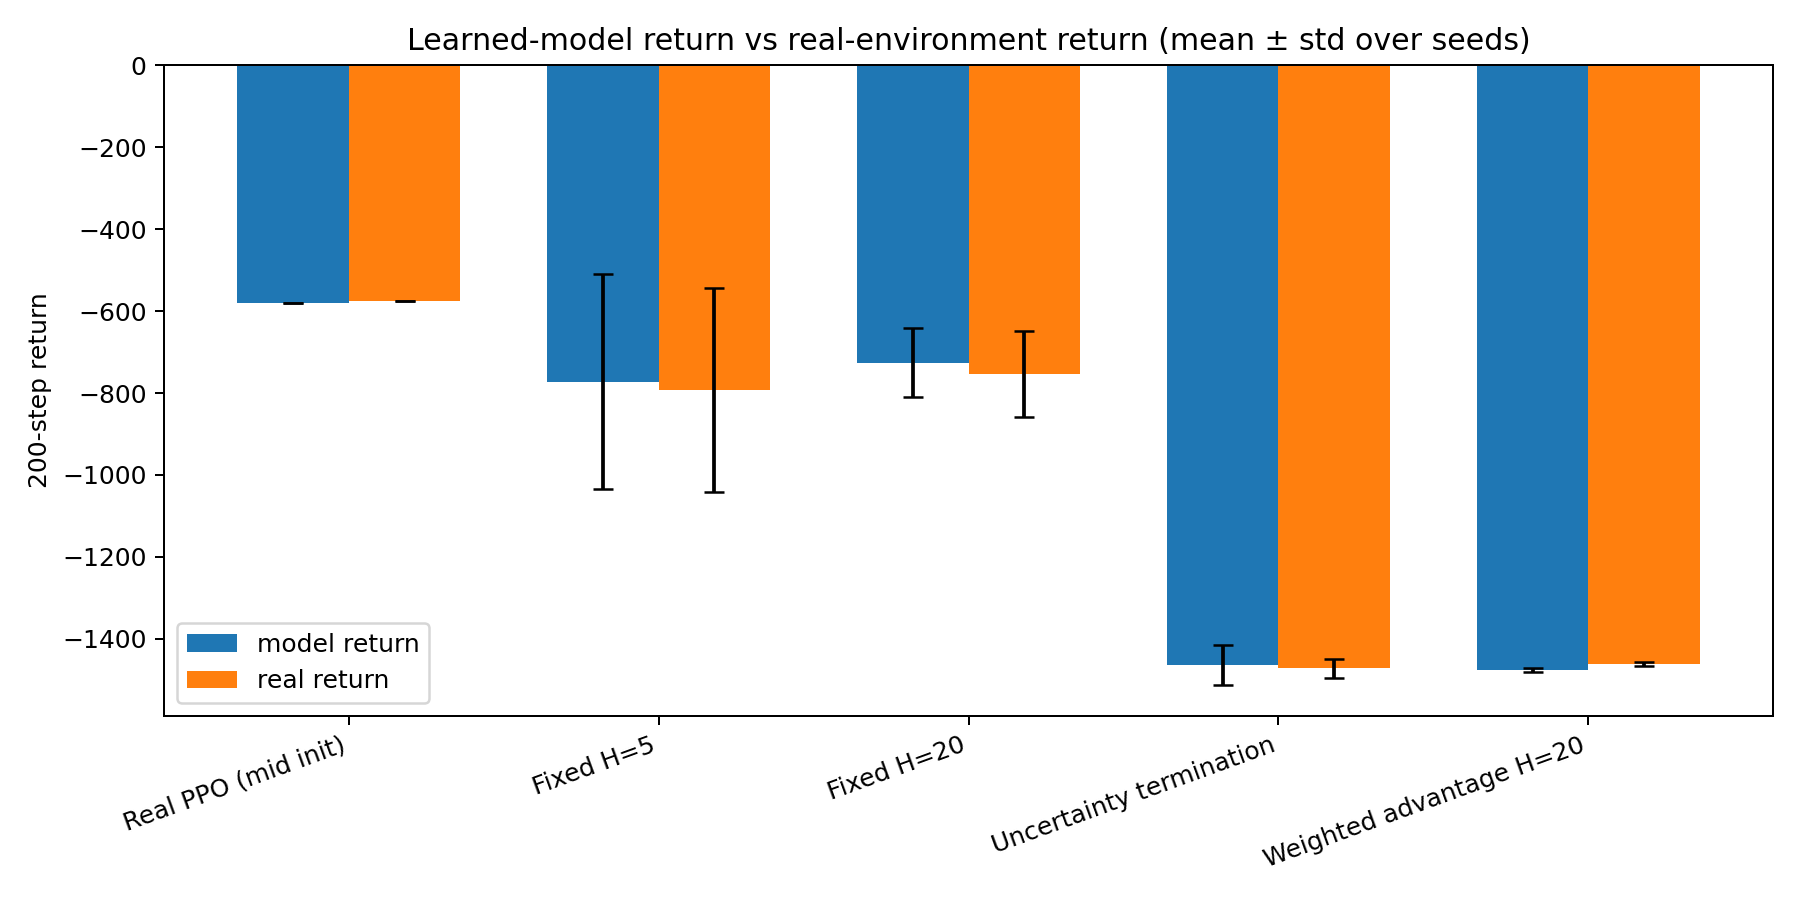
\includegraphics[width=\linewidth]{images/model_vs_real_return_seeds.png}
\caption{Model and environment returns. Error bars for refinement methods show variation across seed means. The shared starting policy has a single checkpoint. The environment is the original Gymnasium simulator.}
\label{fig:returns}
\end{figure}

The stronger-policy comparison starts from the checkpoint that generated the dynamics data and uses approximately 100,000 imagined transitions. It contains one refinement run per method. The starting environment return is $-150.47$. Fixed $H=20$ and uncertainty termination retain returns of $-149.74$ and $-149.83$. Fixed $H=5$ and weighted advantages reach $-295.68$ and $-288.62$. Table~\ref{tab:strong-policy} in the appendix gives the complete recorded comparison.

The existing runs measure the combined effect of the implemented rollout, reward, critic, and optimizer choices. The analytical examples isolate boundary and weighting effects.
